\setcounter{chapter}{-1} % to make this chapter 0
\chapter{Introduction}
\label{chap:introduction}

Rust is a modern systems programming language

\section{Motivation and Background}
\label{sec:motivation}

It is an inevitable fact of software development that the engineer will spend a
substantial amount of their time modifying and improving existing codebases.
Such modifications will range from small bug fixes to complete architecture
overhauls. Regardless of how large (or small) the situation is, refactoring –
systematic restructuring of the codebase without altering its external behaviour
– plays a pivotal role in maintaining code quality and limiting code smell over
time. Despite refactoring being commonplace in many systems programming
languages like C++ or Java, implementing automated refactoring tools remains
challenging, particularly in languages with advanced features and strict safety
guarantees, such as Rust.

When it comes to memory management, two schools of thought have dominated for
the last half-century. One tradition leans on automated techniques like garbage
collection, while the other relies on manual, explicit management. In this
landscape, Rust stands out by enforcing memory safety and concurrency through
its rigorous system of ownership, borrowing, and lifetimes. Yet, the very
features that make Rust safe also introduce massive hurdles for automated
refactoring. A naive, “copy and paste” implementation of extract method
refactoring that works in more forgiving languages like Python and Java will hit
the proverbial brick wall that is the Rust borrow checker. Whilst the borrow
checker and other compilation checks will prevent unintended consequences, the
programmer must now deal with a whole host of other issues.

Against this backdrop, \textit{Adventure of a Lifetime} (AoL)~\cite{aol}
introduced the conceptual framework for automated “Extract Method” refactoring
in Rust. From there, \textit{Borrowing without Sorrowing}~\cite{borrowing}
implemented the concepts outlined in \textit{Adventure of a Lifetime} as an
IntelliJ IDEA plugin. This project now builds on those foundations, aiming to
extend, improve and explore new frontiers for automated Rust refactoring.

\subsection{Do People Actually Refactor?}
\label{sec:do-people-refactor}

Despite widespread agreement on the value of continuous, incremental code
improvements, one might still wonder: do development teams truly refactor in
practice, or is it just an idealized principle? A recent large-scale survey of
1,183 professional developers by the JetBrains team, \textit{One Thousand and
One Stories: A Large-Scale Survey of Software Refactoring}~\cite{jetbrains},
sheds light on this question. The results show that refactoring is
unquestionably a routine part of modern software engineering:

\begin{itemize}
    \item \textbf{Frequent Refactoring:} Over 77\% of surveyed developers
    reported refactoring code at least once a week, with 40.6\% doing so “almost
    every day” and another 36.9\% at least every week.
    \item \textbf{Lengthy Sessions:} Refactoring can be time-intensive; 66.3\%
    of respondents indicated they had spent an hour or more in a single session
    refactoring their code.
    \item \textbf{Rare “Non-Refactorers”:} Only 2.5\% stated that they “never”
    refactor code. Even within that group, many had at least renamed or
    relocated code elements—activities the survey authors classify as
    refactoring.
\end{itemize}

These findings confirm that refactoring is more than just a best-practice
slogan: most teams regularly restructure and clean up their code. At the same
time, the significant number of hour-plus refactoring sessions suggests that
technical debt can build up to a point where larger-scale efforts become
necessary. Understanding how, why, and when developers refactor can thus guide
the design of more effective refactoring tools and strategies.

\subsection{Importance of Refactoring in Software Engineering}
\label{sec:importance-refactoring}

In large projects, codebases can quickly become very unwieldy. Refactoring is a
crucial tool that helps engineers keep the technical debt at a manageable level.
It ensures that system complexity remains manageable by promoting cleaner
abstractions, fewer side effects, and much clearer data flows.

Additionally, whilst refactoring itself doesn’t add new features, it often
uncovers latent defects and unexpected behaviours or side effects. It can be
used to bring clarity to confusing, hundred-plus line methods, and makes testing
significantly more straightforward.

Finally, well-factored code is much easier to understand and thus modify. This,
in turn, will speed up future iterations, feature implementations, and
onboarding of new team members.

\subsection{What is “Extract Method” Refactoring?}
\label{sec:extract-method}

“Extract Method” is a common refactoring technique where a contiguous block of
code (often a few lines or a loop body) is extracted into its own function. The
original code is replaced with a call to this newly created function. By
breaking down the large methods or blocks into smaller, aptly named functions,
readers can far more quickly grasp the purpose of each piece of logic.

In Java or other garbage-collected languages, method extraction is
straightforward: you collect parameters, create a new function, and replace the
original lines with a function call. Rust, however, introduces additional layers
of complexity due to ownership and borrowing. The example below (in Java)
illustrates how this technique works at a superficial level.

\inputminted{java}{Code/refactor_example.java}

\subsection{Why Rust Poses Unique Challenges}
\label{sec:rust-challenges}

\begin{enumerate}
    \item \textbf{Ownership:}
    Each value in Rust has a single owner that governs the value's lifetime.
    Once the owner goes out of scope, the value is dropped. This design
    eliminates many types of memory errors (such as use-after-free), but can
    complicate refactoring: relocating or splitting functionality into separate
    functions may transfer or divide ownership in unexpected ways.

    \inputminted{rust}{Code/ownership_example.rs}

    In the above example, s1 is “moved” into s2, making s1 no longer valid
    afterward. If a refactoring operation was to pass s1 into a function that
    takes ownership, the original owner cannot access it unless ownership is
    returned. Alternatively, we could end up with code that refuses to compile,
    forcing the developer to manually debug and fix the refactored code.

    \item \textbf{Borrowing:}
    Instead of copying or moving data, Rust encourages passing references.
    However, these references can be immutable (\texttt{\&T}) or mutable
    (\texttt{\&mut T}), and only one active mutable reference is allowed at a
    time. When extracting logic into a separate function, it is important to
    ensure that references remain valid and continue to adhere to Rust's
    borrowing rules. The examples below demonstrate how borrowing can be
    effectively handled. However, if multiple references with overlapping
    mutable access are introduced by refactoring, the compiler's rules may
    require parameter signatures or function boundaries to be revised
    accordingly.

    \begin{table}[h!]
        \centering
        \begin{tabular}{@{}p{0.47\textwidth}@{\hspace{0.03\textwidth}}|@{\hspace{0.03\textwidth}}p{0.47\textwidth}@{}}
        \textbf{Immutable Borrow} & \textbf{Mutable Borrow} \\[5pt] \hline \\[-5pt]
        \inputminted[frame=none, linenos=false, breaklines=true, breakanywhere=true]{rust}{Code/borrowing_example_0.rs} &
        \inputminted[frame=none, linenos=false, breaklines=true, breakanywhere=true]{rust}{Code/borrowing_example_1.rs}
        \end{tabular}
    \caption{Immutable and mutable borrowing in Rust}
    \label{tab:borrowing_imm_mut}
    \end{table}

    \item \textbf{Lifetimes and their Management:}
    The Rust compiler tracks how long references live to guarantee memory
    safety. Any function that takes (or returns) references must define or infer
    lifetime parameters. When we write Rust code normally, such as the example
    below, the compiler is capable of inferring these lifetimes for the
    programmer.
    \inputminted[frame=none]{rust}{Code/compiler_lifetime_inference_0.rs}
    When the programmer writes \texttt{echo(message: \&str) -> \&str}, the
    compiler is quietly inferring a generic lifetime for both the parameter and
    the return value. In effect, the compiler treats this as if the programmer
    wrote:
    \inputminted[frame=none]{rust}{Code/compiler_lifetime_inference_1.rs}
    So, behind the scenes, Rust sees that \texttt{message} is a reference that
    lives at least as long as \texttt{'a}, and it infers that the output must
    share that same \texttt{'a} lifetime. The programmer doesn't need to write
    \texttt{<'a>} or annotate the references explicitly, because the language
    automatically applies its lifetime inference rules whenever possible.
    \\ If engineers later extract code into new functions—especially if multiple
    reference parameters or more complex borrowing patterns are involved—the
    compiler might no longer be able to figure out the relationships between
    references, forcing programmers to specify such \texttt{'a} parameters
    explicitly.

    \item \textbf{Non-local Control Flow}
    Rust allows \texttt{return}, \texttt{break}, and \texttt{continue} inside
    code blocks. Extracting a fragment of code containing, for example, an early
    \texttt{return}, into a function changes the flow of control unless handled
    explicitly.
    % TODO Expand on this section
\end{enumerate}

\subsection{Adventure of a Lifetime: Automated Refactoring for Rust}
\label{sec:aol}

A foundational contribution toward automated refactoring for Rust was made by
Sergey et al.\ in \textit{Adventure of a Lifetime}~\cite{aol}. While ``Extract
Method'' refactoring is relatively straightforward in languages like Java, the
challenges discussed in the previous section demonstrate why a similar algorithm
for Rust is far from trivial. To tackle these unique challenges,
\textit{Adventure of a Lifetime} introduced a specialized refactoring framework
tailored to Rust’s complexities.

Their approach addressed Rust-specific issues using multiple specialized passes.
For example, one pass systematically encodes \texttt{return}, \texttt{break},
and \texttt{continue} statements into an auxiliary enum, allowing the caller
function to reconstruct the original control flow by matching on variants such
as \texttt{Ok(...)}, \texttt{Return(...)}, etc. Another pass utilizes
constraint-based ownership analysis to precisely determine and assign the
correct ownership levels (owned or borrowed references) to variables involved in
extracted code fragments.

The systematic handling of these issues ensures correctness with respect to
ownership, borrowing, and lifetimes, thereby overcoming the primary hurdles
faced when naively transferring techniques from languages like Java directly
into Rust. Figure \ref{fig:aol_process} from \textit{Adventure of a Lifetime} outlines the complete
refactoring process.

\begin{figure}[H]
    \centering
    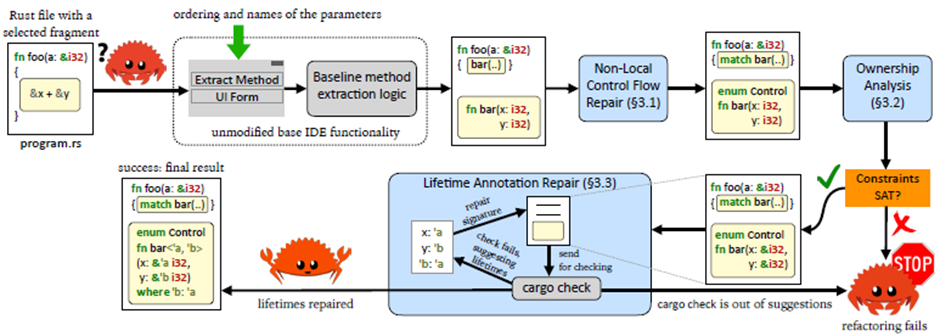
\includegraphics[width=0.8\textwidth]{Figures/AoL_algorithm.png}
    \caption{The refactoring process as outlined in \textit{Adventure of a Lifetime}}
    \label{fig:aol_process}
\end{figure}

The authors implemented this approach as \textit{Rusty Extraction Maestro} (REM)
on top of IntelliJ IDEA’s Rust plugin. Their empirical evaluation on multiple
real-world Rust projects demonstrated that REM handles a wider range of
extractions than existing IDE tools, including scenarios involving multiple
borrows and nested references. Specifically, REM successfully managed 37 out of
40 tested cases, outperforming both IntelliJ IDEA alone and VSCode’s Rust
Analyzer. The study also showed that REM-generated functions extracted quickly
(on the order of one to two seconds), making it practical for everyday
development. Most of the overhead arose from repeated calls to \texttt{cargo
check}, although the delay remained acceptable for typical usage scenarios.

However, the evaluation also identified several limitations. REM struggles with
code involving complex generics or elaborate trait bounds due to limited type
inference capabilities in IntelliJ's Rust support. Additionally, it lacks
support for asynchronous programming constructs (\texttt{async}/\texttt{await})
and is unable to correctly extract functions that partially move struct fields.
Macros beyond standard-library macros frequently disrupt refactoring attempts.
Lastly, REM requires (and also assumes) a compilable project state, as it
requires compilation checks to aid with its analysis. It often generates
functions with overly verbose type signatures due to explicit lifetime and
ownership annotations, despite the application a robust set of lifetime elision
rules.

\section{Problem Statement}
\label{sec:problem-statement}

\subsection{Issues with Existing Automated Refactoring Tools}
\label{sec:issues-existing-tools}

Rust's unique ownership, borrowing, and lifetime system presents challenges that
traditional refactoring tools don't typically encounter. In languages like Java
or Python, transformations such as ``Extract Method'' can be applied directly
with minimal risk of breaking the code. However, Rust's strict guarantees mean
that naïvely lifting code into a new function often results in compilation
errors or unintended changes in behavior due to ownership conflicts, borrowing
rules, or lifetime mismatches. As a result, programmers often have to manually
fix the refactored code—a process that can take significantly longer than
rewriting it from scratch. While automated refactoring tools for Rust, such as
RustRover and the IntelliJ Rust plugin, handle simple extractions well, they
struggle with more complex constructs due to these inherent language
constraints.

For instance, IntelliJ IDEA's Rust plugin and Visual Studio Code's Rust Analyzer
both handle simpler scenarios—like extracting a small code block without complex
borrows—but rely heavily on IntelliJ's type inference or \texttt{rustc}. They
often provide incomplete coverage for features such as
\texttt{async}/\texttt{await}, generics with intricate trait bounds, or macros,
leading the tools either to produce incorrect code or to refuse to recognize an
extraction altogether. Moreover, these tools commonly struggle with non-local
control flow, such as an early \texttt{return} from deep within a nested block.

By contrast, REM specifically targets these Rust-specific pain points. First, it
applies a specialized ownership analysis algorithm that determines exactly how
data should be passed—owned versus borrowed—in an extracted method. Second, it
reifies non-local control flow operations like \texttt{return}, \texttt{break},
and \texttt{continue} by translating them into a custom enum and then patching
the call-site logic. Finally, REM refines the resulting function's lifetime
annotations in a loop, using \texttt{cargo check} to repeatedly gather compiler
feedback. This structured approach greatly expands the variety of Rust code
patterns that can be safely refactored.

However, REM has several limitations. It heavily depends on the IntelliJ IDEA
plugin for Rust, which is outdated and no longer supported. Additionally, it
relies on numerous undocumented and rapidly changing \texttt{rustc} internals,
leading to frequent build issues as third-party packages update and become
incompatible. Another major drawback is that REM can only refactor code that
compiles, as it relies on \texttt{cargo check}, which still requires successful
compilation. Lastly, it passes multiple temporary files around on disk, making
it incompatible with tools like \texttt{rust-analyzer}, which operate entirely
in memory through the Language Server Protocol.

\subsection{Need for Verification}
\label{sec:need-verification}

An automated refactoring toolchain is only as good as its ability to preserve
the program's behavior. Rust refactoring poses particular challenges here due to
its strict ownership and lifetime rules. A good refactoring must ensure that the
transformed program maintains the exact observable behavior as before. Although
comprehensive test coverage is the primary practical means of ensuring the
preservation of functionality, tests are often slow and limited—they identify
only \textit{that} a problem exists, not precisely \textit{where} it was
introduced.

Verifying semantic preservation after transformations is notoriously
challenging, particularly in Rust. Rust's unique language features complicate
semantic preservation proofs or automated verification techniques. Moreover,
Rust code produced by REM may include constructs—such as enums for reified
control flow or explicit lifetime annotations—that can appear unfamiliar or
unnecessarily complex to human readers. While this complexity does not imply
semantic changes, confirming correctness remains essential. Therefore, employing
rigorous semantic validation (automated, partial, or manual) alongside
refactoring is necessary to ensure transformations remain safe, accurate, and
reliable.

\section{Project Aims and Objectives}
\label{sec:project-aims}

This project seeks to improve and extend the capabilities of the \texttt{Rusty
Extraction Maestro (REM)} tool while making the refactoring process more
accessible and verifiable. Specifically, the aims can be grouped into three key
areas: enhancing \texttt{REM}’s standalone functionality, establishing a solid
approach to verifying refactorings, and developing a proof-of-concept
\texttt{VSCode} extension. A long-term ambition is to explore potential
integration with \texttt{Rust Analyzer} if future architectural changes permit.

\subsection{Improve and Extend \texttt{REM}}
\label{sec:improve-extend-rem}

A principal goal is to remove \texttt{REM}’s existing dependencies on both
\texttt{rustc} and IntelliJ IDEA, allowing the tool to function independently.
By offering a standalone solution, \texttt{REM} would be simpler to incorporate
into various workflows, free of the overhead or version constraints tied to
external IDEs and compilers. This will be achieved through a single
comprehensive CLI that links all stages of \texttt{REM} together.

To ensure broader adoption, another focus is to provide \texttt{VSCode}
integration in the form of a user-friendly plugin. This plugin should install
easily, require minimal setup, and offer automated \texttt{Extract Method}
support for Rust directly in Visual Studio Code. In parallel, the project aims
to expand \texttt{REM}’s capabilities to handle advanced Rust features, such as
\texttt{async/await} constructs, macros, closures, \texttt{const} functions, and
more intricate generics. Addressing these challenging language constructs will
make \texttt{REM} suitable for a greater variety of real-world Rust codebases.

\subsection{Verification of \texttt{REM} / Refactorings}
\label{sec:verification-rem}

Automated refactorings are only meaningful if they preserve the program’s
original semantics. While typical “copy-and-paste” style transformations rarely
alter program logic, \texttt{REM}’s deeper rewrites---which may include lifetime
adjustments or reified control-flow enums---require stronger assurances that the
resulting code truly behaves as intended. To achieve this, the project intends
to develop a theoretical framework (or algorithm) for proving equivalence
between the original and refactored code.

An emerging strategy involves functional translation---moving refactored Rust
code into a simpler, more mathematically tractable language subset or an IR for
proof purposes. Recent development to toolchains like
\texttt{CHARON}\cite{charon} and \texttt{AENEAS}\cite{aeneas} can assist by
allowing for a complete translation of a Rust program into a set of functional,
proof oriented languages like \texttt{F*} and \texttt{Coq}. Though complete
verification of all Rust code remains infeasible due to the language’s evolving
semantics, partial or scenario-specific proofs can still bolster confidence in
\texttt{REM}’s correctness. Demonstrating a handful of end-to-end
examples---from extraction in Rust to verified equivalence in a proof
assistant---will illustrate the viability of this approach. Moreover, the
verification pipeline has the potential to be integrated into the main body of
\texttt{REM}, providing the programmer with a guarantee that their code’s
functionality hasn’t been affected or alternatively, the verification tool can
be leveraged to execute a comprehensive series of case studies that further
validate \texttt{REM}’s functionality.

\subsection{Build a Proof-of-Concept Extension for \texttt{VSCode}}
\label{sec:vscode-extension}

A strong emphasis is on producing a proof-of-concept \texttt{VSCode} extension
that showcases \texttt{REM} in action within one of the most commonly used Rust
development environments. This extension should seamlessly integrate into a
developer’s normal workflow, from code editing to debugging, without burdensome
setup. By offering an easy-to-install plugin, the refactoring workflow becomes
more accessible, and potential refinements can be validated in real-world coding
sessions.

A core demonstration will involve extracting method fragments in a variety of
Rust files and showing how the extension generates well-typed,
behavior-preserving code. The key detail here is that \texttt{REM} relies on its
new, standalone core, instead of a platform or program specific implementation.

\subsection{Potential for the Long Term Goal of Merging \texttt{REM} with
\texttt{Rust Analyzer}}
\label{sec:long-term-goal}

Finally, looking beyond the immediate development schedule, an intriguing
possibility is merging \texttt{REM}’s functionality with \texttt{Rust Analyzer},
the official language server for Rust. \texttt{Rust Analyzer} already converts
source code into an intermediate representation to power syntax highlighting,
code completion, and basic refactorings. If \texttt{REM} can leverage that IR,
it might inject advanced lifetime analysis and partial verification steps
directly into the analyzer pipeline.

However, \texttt{Rust Analyzer} is deliberately kept lightweight and
incremental, while \texttt{REM} aspires to be a comprehensive solution that
tackles complex rewriting tasks. Hence, if integration proves overly burdensome,
a compromise could be to develop a stripped-down subset of \texttt{REM} for
merging. This long-term exploration depends on how \texttt{Rust Analyzer}
evolves and whether the Rust community adopts more sophisticated refactoring
workflows within a single unified environment. The alternative solution of a
standalone \texttt{VSCode} extension designed to be used alongside \texttt{Rust
Analyzer} is also seen as acceptable in this case.
